%!TEX TS-program = xelatex
%!TEX encoding = UTF-8 Unicode

\documentclass[12pt, a4paper]{article}

%% Page Layout
\usepackage[margin=1in]{geometry}

\usepackage{euler} % math font package needs to be loaded before others
\usepackage{xunicode,xltxtra, polyglossia}
\setdefaultlanguage[variant=american]{english}

%% fonts, symbols, text
	%%% fonts
	\usepackage{fontspec} %(include if mathspec is not loaded)
	\defaultfontfeatures{Mapping=tex-text, Ligatures=TeX}
	%%% text decoration
	\usepackage[normalem]{ulem} % sout
	%%% semantics symbols
	\usepackage{stmaryrd}
	\usepackage{amsmath,amssymb}
	\newcommand{\transl}{\rightsquigarrow \ensuremath}
	%%% other symbols
	\usepackage{pifont}% http://ctan.org/pkg/pifont
	\newcommand{\cmark}{\ding{51}}%
	\newcommand{\xmark}{\ding{55}}%

%% layout
%%% page layout
\usepackage{multicol}


%% bibliography
\usepackage[round]{natbib}
\newcommand{\posscite}[1]{\citeauthor{#1}'s (\citeyear{#1})}

%% figures, examples, diagrams
%%% examples
\usepackage{linguex}
\renewcommand{\firstrefdash}{}
%%% tables 
\usepackage{booktabs}
%%% figures
\usepackage{graphics}


%% decoration and features
%%% colors
\usepackage[dvipsnames]{xcolor}

%% bibliography
\renewcommand*{\refname}{\normalsize\textbf{References}\\ \vspace{-.5\baselineskip}}

%% fonts
\setmainfont[Scale=MatchLowercase,Mapping=tex-text, SmallCapsFeatures={Letters=SmallCaps}]{Times New Roman}
\setsansfont[Scale=MatchLowercase,Mapping=tex-text]{Times New Roman}

\usepackage{setspace}

\newcommand{\citepos}[1]{\citeauthor{#1}'s \citeyear{\#1}}
\newcommand{\citeposs}[1]{\citeauthor{#1}'s}
\newcommand{\citetpos}[1]{\citeauthor{#1}'s (\citeyear{\#1})}

\parindent=2ex

\begin{document}

\bibliographystyle{plainnat}
% \enablehyphenation
% \vspace{-2em}
% \maketitle

\begin{center}
	\textbf{\large%\thetitle
		%A diverse family (of sentences)\\ 
		Projection differs across embedding operators---but not like you think}
\end{center}

\vspace*{-.8\baselineskip}
\noindent 
	We present experimental evidence \textbf{(i)} that the projection of the content of attitude complements varies across four entailment-canceling operators (negation, question, modal, antecedent of conditional) and \textbf{(ii)} that this by-operator variation differs across attitude predicates. Our results do not align with the long-standing distinction between factive and semi-factive predicates (see, e.g., \citealp{karttunen_observations_1971,hooper_applicability_1973,djarv_cognitive_2018}). Instead, the observed by-operator variation groups predicates by lexical semantic/pragmatic properties that raise important questions for future research on projection.

\noindent
	{\bf Projection across entailment-cancelling operators.} Interpreters may infer that a speaker who utters one of the attitude ascriptions in  \ref{ex:family} is committed to the truth of the content of the complement (CC),
	% that Julian dances salsa,
	even though it occurs under an entailment-canceling operator, such as negation \ref{ex:neg}, a polar question \ref{ex:q}, a modal \ref{ex:mod}, or a conditional \ref{ex:cond}.

	%	Certain attitude ascriptions come with an inference to the truth of their complement, even if embedded under entailment-cancelling operators (shown for \emph{discover} in \ref{ex:family}), in which case the inference is said to \emph{project} (e.g. \citealp{karttunen_observations_1971}).

	\vspace{-.3\baselineskip}
	\ex. \label{ex:family}
		\a. \label{ex:neg}
			Negation: \hfill
			\emph{\lq Cole didn't discover that Julian dances salsa.\rq}
		\b. \label{ex:q}
			Polar Question: \hfill
			\emph{\lq Did Cole discover that Julian dances salsa?\rq}
		\c. \label{ex:mod}
			Modal: \hfill
			\emph{\lq Perhaps Cole discovered that Julian dances salsa.\rq}
		\d. \label{ex:cond}
			Conditional: \hfill
			\emph{\lq If Cole discovered that Julian dances salsa, Logan will be joyful.\rq}
		\z.
	\z.

	\vspace{-.4\baselineskip}
	% Previous work on projection showed that it is not a categorial property of lexical triggers \citep{tonhauser_how_2018}, but a gradient one, affected by various contextual factors \citep{simons_what_2010,de_marneffe_did_2012,beaver_questions_2017,degen_prior_2021}. In light of this, we expect that the hetergeneous entailment-cancelling operators in \ref{ex:family} affect projection differentially.
	%
	\citet{karttunen_observations_1971} proposed that the CC of factive predicates (e.g. \emph{regret, forget}) projects from under all four operators, whereas that of semi-factive predicates (e.g. \emph{discover, realize, see, notice}) always projects from under negation, but not always from under polar questions, modals, or conditionals. 
	
	There has been, to date, one investigation of by-operator variation: \citet{smith_relationship_2014}, who investigated by-operator projection variation for negation and conditional embeddings, observed that there is by-operator variation for some contents (e.g., that of \emph{know}, but not that of clefts) and that this by-operator variation differs across contents: The content of NRRCs and \emph{win} was more projective under conditionals than negation, the opposite pattern was observed for \emph{know} and epithets. However, the response task they used asked participants to rate how surprised they would be to learn the content under investigation after observing the utterance. Since factors other than speaker commitment modulate surprisal, it is not clear that they (only) measured projection.

	There has not yet been an experimental investigation of by-operator variation between factive and semi-factive predicates. \citet{djarv_cognitive_2018} and \citet{tonhauser_how_2018} did, however, observe by-predicate projection variation in polar questions. \citet{djarv_cognitive_2018} found a difference between \emph{be happy} and \emph{appreciate} (which they assumed are factive predicates) and \emph{be aware} and \emph{realize} (which they assumed are semi-factive predicates). However, the response task (acceptability of an affirmation of the main clause while the CC was denied) did not measure projection of the CC. \citealt{tonhauser_how_2018} measured projection of the CC of a broad range of attitude predicates from under polar questions: The by-predicate projection differences they observed did not align with what would be expected from Karttunen's classification (e.g., the CC of semi-factive \emph{realize} was as projective as that of factive \emph{be annoyed} and more projective than that of semi-factive \emph{discover}).

	\noindent
	{\bf Experiment.} We present the results of an experiment designed to investigate by-operator projection variation for the CCs of 20 attitude predicates, including purported factive and semi-factive predicates (e.g., \emph{be annoyed, discover}). Projection was measured for the same contents across all four operators in \ref{ex:family} using the `certain that' diagnostic for projection (see also, e.g., \citealt{tonhauser_how_2018,djarv_prosodic_2017, mahler2020}). 


	%In our work, we analyze measures from a task designed to measure speaker commitment more directly to address the questions: \textbf{(i)} Is projection affected by differences in entailment-canceling environments? \textbf{(ii)} Do these effects vary for different triggers (and in what way)? We used a response task to elicit judgments about how strongly a speaker would be committed towards the embedded clause \citep[from][]{tonhauser_prosodic_2016}. We presented sentences like in \ref{ex:family} as asserted by a named speaker (e.g. “\textbf{Daniel:} \emph{\lq Did Cole\dots?\rq}”). Participants then provided a certainty-rating in response to a prompt like: \emph{“Is Daniel certain that Julian dances salsa?”}, by moving a slider on a scale from \lq no\rq\ (coded as \texttt{0}), to \lq yes\rq\ (coded as \texttt{1}). 

% paragraph experiment (end)
\noindent
{\bf Methods and expectations.}
	Projection of the CC of the 20 attitude predicate was measured in four sets of experiments: The attitude predicates were embedded under polar questions in Exps.~1, under negation in Exps.~2, under {\em perhaps} in Exps.~3, and in the antecedent of a conditional in Exps.~4. (Each set of experiments consisted of three experiments that differed in the at-issueness measure used in a separate block. We focus on the projection ratings here.) In each experiment, participants were asked to read utterances like those in \ref{ex:family} and judge whether the speaker (who was named) was certain of the CC (e.g.: Is [the speaker] certain that Julian dances salsa?). Participants gave their response on a slider marked `no' (coded as 0) at one and and `yes' (coded as 1) on the other end. Each participant rated the projection of the CC of all 20 attitude predicates (each paired with a unique content from a set of 20 contents) under one operator. We analyze the data from 2,682 self-reported native speakers of American English recruited on Prolific or Amazon's MT platform. We expect the CC of factive predicates to consistently receive relatively high projection ratings under all four operators, and the CC of semi-factive predicates to exhibit high projection ratings under negation and possibly lower ratings under the other operators. 

	%We compared certainty-ratings for the four entailment-canceling operators in \ref{ex:family}, and 20 clause-embedding predicates (\texttt{verb}: {\em be annoyed, discover, know, reveal, see, acknowledge, admit, announce, confess, confirm, establish, hear, inform, prove, pretend, suggest, say, think, be right, demonstrate}).
	%	Based on the Karttunen-Djärv generalization about emotive factives vs. cognitive semi-factives, we would expect emotive factives (\emph{be annoyed}), and verbs normally taken to be factive (\emph{know}), to be highly projective in a way that is indifferent to the embedding context, and cognitive semi-factives (\emph{discover, see}) to show higher projectivity ratings under negation compared to questions and conditionals.

	%The study, originally designed to address a different research question, consisted of 12 experiments, all of which manipulated the factor \texttt{verb} for 20 items corresponding to to the content of the complement clause. Experiments 1--3 used polar question embedding, exps. 4--6 used negation, 7--9 modals, and 10--12 conditionals, making the \texttt{operator} manipulation a between-subjects factor. 

	%We analyzed data from 2682 self-identified native English speakers participated online across the 12 experiments (recruited via Prolific and Amazon MTurk). Participants saw items Latin-squared and randomized with six control stimuli.

	% paragraph method (end)

\noindent
{\bf Results.}
	Fig.\ref{fig:figure1} shows the mean projection ratings for the 20 attitude predicates by embedding operator; the predicates are ordered by their mean projection across all operators (\emph{be annoyed} has the highest overall projection mean). We observe by-operator variation in projection means as well as differences across the predicates in by-operator variation: For instance, whereas the CC of \emph{be annoyed} projects more from under negation (and questions) than from under conditionals and modals, the CC of \emph{know} projects less from under negation than under questions, but more from under negation than from under modals, and the CC of \emph{discover} projects less from negation than from under conditionals and questions, and more from under negation than modals. These results (which are supported by linear mixed effects models, see Table \ref{t:models}) are not aligned with the distinction between factive and semi-factive predicates proposed in \citealt{karttunen_observations_1971} or assumed in \citealt{djarv_cognitive_2018}: Contrary to assumption, the CC of the purportedly factive predicate \emph{be annoyed} does not project invariably from all four operators, and the CC of the purportedly semi-factive predicate \emph{discover} does not project more from under negation than the other three operators. For {\em know}, we observe a third pattern, one that is neither that of a factive nor that of a semi-factive predicate. Similar considerations apply to \emph{see} and \emph{reveal}, which are also considered (semi-)factive in the literature.

	% \vspace{-.3\baselineskip}
	% \textbf{version w baseline know/m}
	% \noindent The data was analyzed using a mixed effects linear regression (using \texttt{lme4, lmertest} in \texttt{R}; \citealp{bates_fitting_2015,kuznetsova_lmertest_2016,r_core_team_r_2014}), with \texttt{know} and \texttt{modal} as reference levels, and random intercepts for participants and items. We found highly significant main effects of \texttt{operator} (\texttt{conditional}: $+0.142$, \texttt{negation}: $+0.143$, ; \texttt{question}: $+0.225$, where $p < 2e^{-16}$ in all three cases), as well as many interactions of \texttt{operator} and  \texttt{verb} across the board (where $p < 0.001$ in $38$ cases, $p < 0.01$ in one, and $p < 0.05$ in three out of $57$ possible interactions).\\

	%	\noindent The data was analyzed using a mixed effects linear regression (using \texttt{lme4, lmertest} in \texttt{R}; \citealp{bates_fitting_2015,kuznetsova_lmertest_2016,r_core_team_r_2014}), with \texttt{be\_annoyed} and \texttt{negation} as reference levels, and random intercepts for participants and items.
		% The mean for this baseline (intercept) is $0.867$.
	%	We found highly significant main effects of \texttt{operator}: For our baseline \texttt{be\_annoyed}, both \texttt{conditional} and \texttt{modal} are clearly less projective than negation, thereby supporting the claim that the embedding context does matter. We also found many interactions of \texttt{operator} and \texttt{verb} across the board, suggesting that the effect of embedding context diffes by verb. Notably, \emph{\lq discover\rq} is more projective in polar questions and conditional antecedents than under negation, patterning opposite to Karttunen's claims about semi-factives. For the emotive predicate \emph{\lq be annoyed\rq} no significant effect is found for \texttt{question} (vs \texttt{negation}), as would be expected based on Karttunen, but we do find unexpected differences between \texttt{negation} $>$ \texttt{conditional, modal}. \emph{know} shows effects that would be incompatible with a characterization as either factive or semi-factive: $\texttt{question} > \texttt{conditional, negation} > \texttt{modal}$. If \emph{\lq know\rq} is a factive predicate, no difference would be expected. If it is semi-factive, we would, again, expect higher projectivity under negation than in questions and conditionals.
	


	% for \texttt{conditional} ($-0.116$, $p < 1.6e^{-13}$) and \texttt{modal} ($-0.156$, $p < 2e^{-16}$), while the effect of \texttt{question} was only marginally significant ($+0.025$, $p < 0.1$). We also found many interactions of \texttt{operator} and \texttt{verb} across the board (where $p < 0.001$ in $43$ cases, $p < 0.01$ in three, and $p < 0.05$ in one out of $57$ possible interactions).\\
	
% paragraph results (end)

\noindent
{\bf Discussion:  Empirical and theoretical implications.} 
Our results --- that projection is modulated by entailment-canceling operators and that there is by-predicate variation in the effect of operator on projection --- have several empirical and theoretical implications. First, the results for the predicates typically considered (semi-)factive, namely \emph{be annoyed, know, see, discover} and \emph{reveal}, call into question the assumed distinction between factive and semi-factive predicates (see also \citealt{beaver_have_2010}). Future research that appeals to these two categories must clarify their definition. Second, claims about projection variability must be relativized to the entailment-canceling operator. While our data replicate the result from \citealt{tonhauser_how_2018} that, in a polar question, the CC of \emph{discover} is less projective than that of \emph{know}, this result does not carry over to conditionals. Finally, our results provide further support (from embedding under negation, modals, and conditionals) for the result of \citealt{degen_are_2022}, that projection does not categorically distinguish between (semi-)factive and non-factive predicates: The CCs of \emph{inform} and \emph{acknowledge}, for instance, are at least as projective as that of some (semi-)factive predicates.
	
\noindent
{\bf Discussion: Novel research question.} Can the observed interaction between predicate and operator in mean projection ratings be predicted from lexical semantic/pragmatic properties of the predicates, and, if so, how? This is a pressing question for future research, to which our data offer some tentative answers. We identify four major patterns. The predicates \emph{pretend} and \emph{think} exhibit the {\bf `Negation high'} pattern, shown in panel (a) of Fig.\ref{fig:figure2}: We tentatively hypothesize that negation (but not the other operators) interacts with the semantic or pragmatic antiveridicality contributed by these predicates. For \emph{announce, confess, admit}, and \emph{reveal}, the CC is most projective when embedded in the antecedent of a conditional: This {\bf `Conditional high'} pattern, shown in panel (b), may suggest that the discourse effect of a conditional interacts with the change-of-state communication predicates. The inferential predicates \emph{prove, confirm}, and \emph{establish} exhibit a {\bf Negation low'} pattern, shown in panel (c): Here, we tentatively hypothesize that the veridical meaning component interacts with negation (but not operators), to result in lower projection ratings under negation. Finally, the predicates  \emph{inform, know}, and \emph{be annoyed} exhibit a {\bf `Modal low'} pattern, shown in panel (d). The lexical meaning of these predicates, whose CCs are among the most projective, appears to interact with the modal adverb {\em perhaps}, yielding lower projection ratings.


	In spite of a lack of categorical distinctions about the projection behavior of our verbs, we can find some interesting patterns. Fig.~\ref{fig:figure2} gives the mean certainty ratings for the four operators by verb, for some groups of our verbs that group together in the way that they show by-operator variation. We highlight four \lq projection-profiles\rq here: the verbs \emph{pretend, think} are the only verbs that are most projective under negation compared to all other operators (\texttt{N} $>$ \texttt{M, Q, C}). \emph{annouce, confess, admit,} and \emph{reveal} are most projective under conditionals, while there is also a tendency that there is more projection from questions compared to modals and negation, a difference that may not be robust for \emph{announce} (\texttt{C} $>$ \texttt{Q} \textcolor{gray!40}{$>_?$} \texttt{M, N}). \emph{prove, confirm,} and \emph{establish} are more projective under modals and conditionals than under questions and negation (\texttt{M, C} $>$ \texttt{Q, N}). Finally, \emph{inform} and \emph{know} are most projective under questions, and least projective under modals (\texttt{Q} $>$ \texttt{N, Q} $>$ \texttt{M}).

	The picture that emerges is complex and requires a nuanced view of lexical effects on projection. I raises the question of how lexical differences between verbs could explain why certain verbs project more from under certain operators and less from others. While much previous work on this question has based their generalizations on impressionistic judgments, empirically establishing different projection-profiles associated with verbs therefore provides a basis for future research on lexical effects on projection.




\newpage

\begin{figure}[h]
	% \vspace{-\baselineskip}
	\centering
	\scalebox{.9}{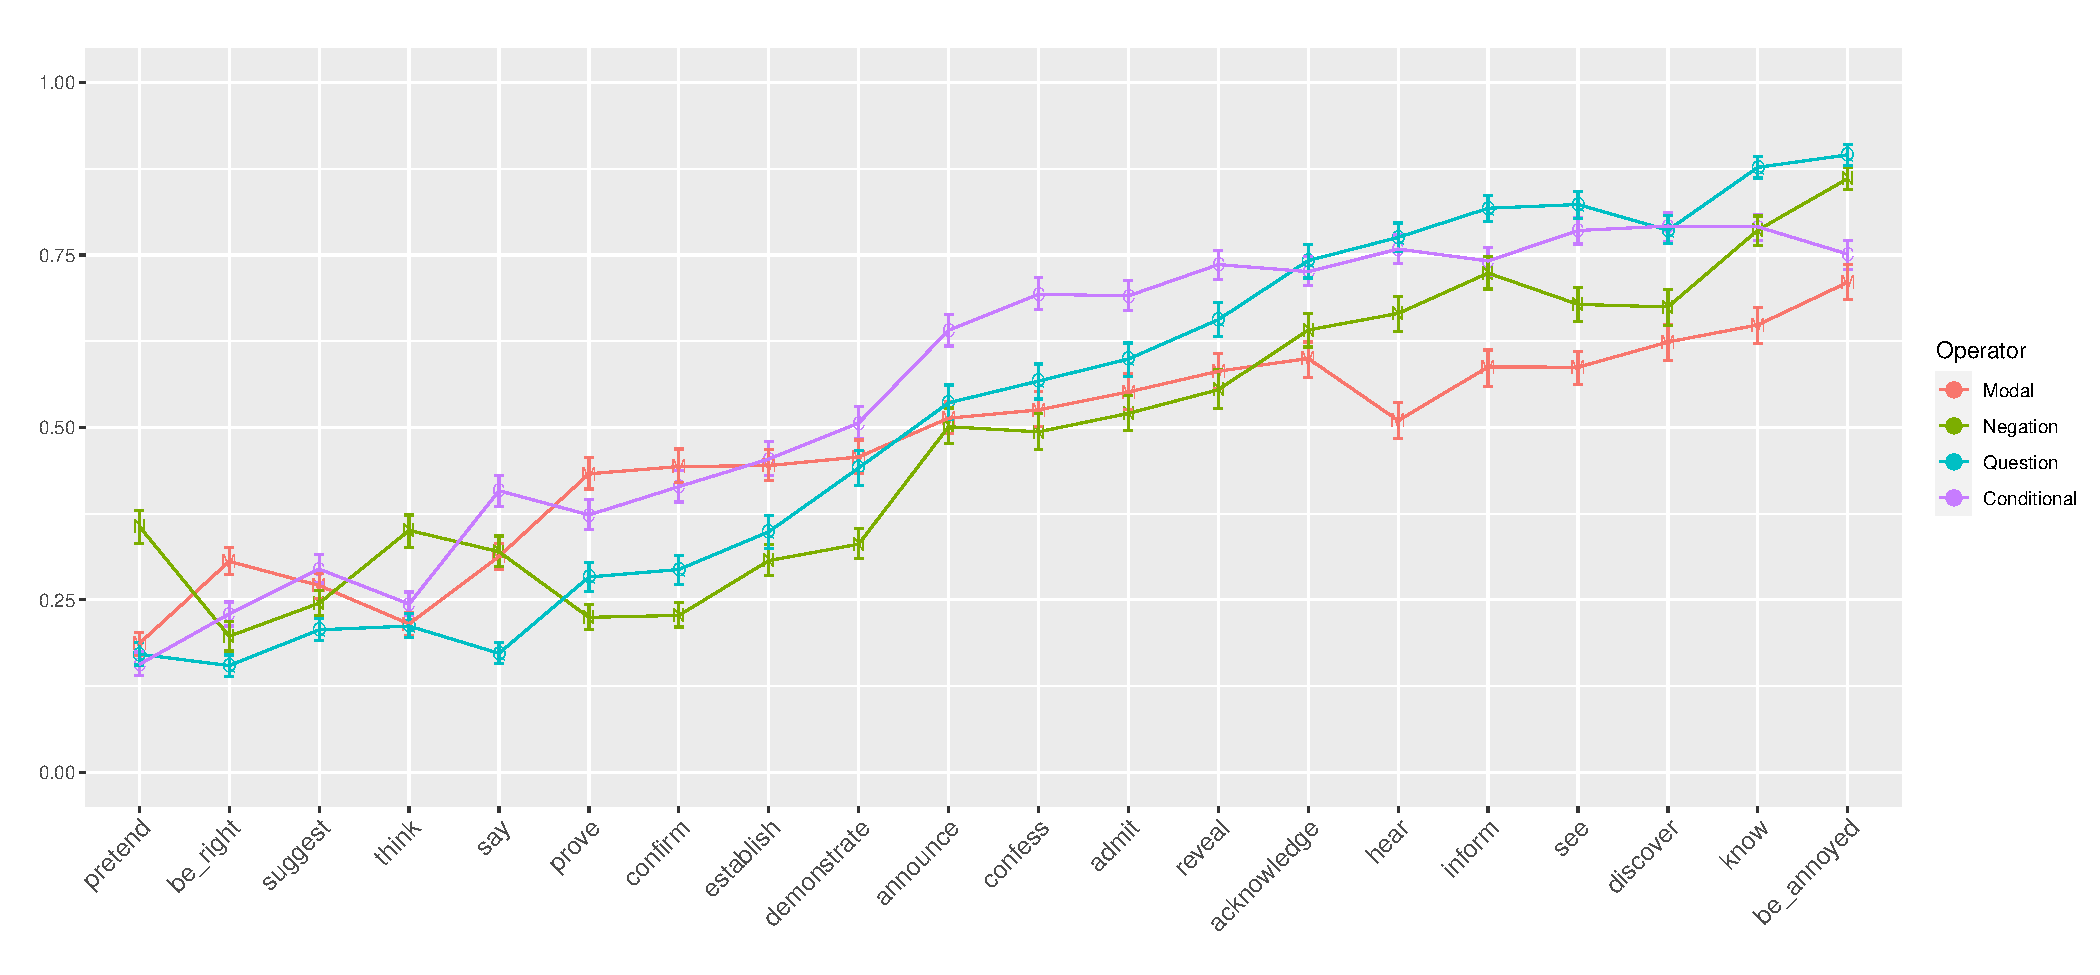
\includegraphics[width=\textwidth]{graphs/proj-by-both.pdf}}\vspace{-1.7\baselineskip}
	\caption{\small Mean certainty ratings by predicate and operator with 95\% bootstrapped confidence intervals. Embedding operator coded by letter and color:  \texttt{N} (blue): negation, \texttt{M} (green): modals, \texttt{C} (red): conditional antecedents, \texttt{Q} (purple): polar questions.}
	\label{fig:figure1}
\end{figure}

\begin{table}[h]
	\centering
	\vspace{-.7\baselineskip}
	\scalebox{.85}{
		\begin{tabular}{llrrrr}
			Model & & Estimate & Std. Error & t-value\\
			\midrule
			\#1 & Intercept: \emph{\bf be annoyed}/negation & 0.87 & 0.01  & 75.8 & *** \\
			& operator: conditional & -0.12 & 0.02  & -7.38 & *** \\
			& operator: modal & -0.16 & 0.02  & -10.04 & *** \\
			& operator: question & 0.02 & 0.01  & 1.74 & n.s. \\
			\midrule
			\#2 & Intercept: \emph{\bf know}/negation & 0.79 & 0.01 &  69.24 & *** \\
			&		operator: conditional & -0.001 & 0.02  & -0.08 & n.s. \\
			&		operator: modal  & -0.14 & 0.02  & -9.2 & *** \\
			&		operator: question & 0.08 & 0.01  & 5.72 & *** \\
			\midrule
			\#3 & Intercept: \emph{\bf discover}/negation & 0.68 & 0.01  & 59.48 & *** \\
			& operator: conditional & 0.11 & 0.02  & 7.11 & *** \\
			&		operator: modal & -0.06 & 0.02  & -3.6 & *** \\
			&		operator: question & 0.1 & 0.01  & 7.07 & *** \\

			\bottomrule
		\end{tabular}
	}
	\vspace{-.3\baselineskip}
	\caption{\small Relevant parts of three linear mixed effects models that predict certainty ratings from a fixed effect of operator, predicate, and their interaction, with random effects for participant and CC. Models were fit with \texttt{lme4, lmertest} in \texttt{R}; \citealp{bates_fitting_2015,kuznetsova_lmertest_2016,r_core_team_r_2014}.}\label{t:models}
\end{table}

\begin{figure}[h]
	\hspace{-2em}
	\begin{minipage}{1.1\textwidth}\centering
		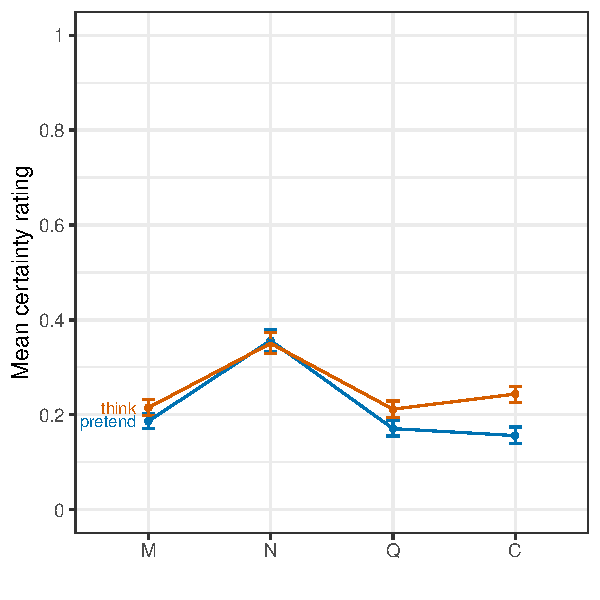
\includegraphics[width=.24\linewidth]{graphs/profile1.pdf}
		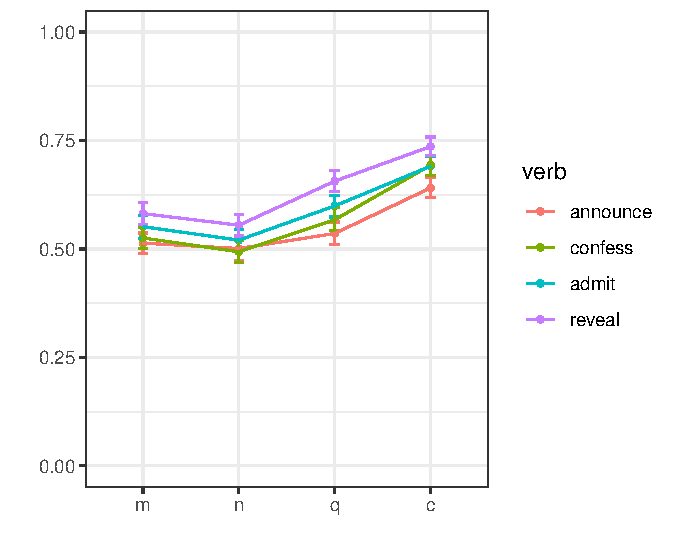
\includegraphics[width=.24\linewidth]{graphs/profile2.pdf}
		% 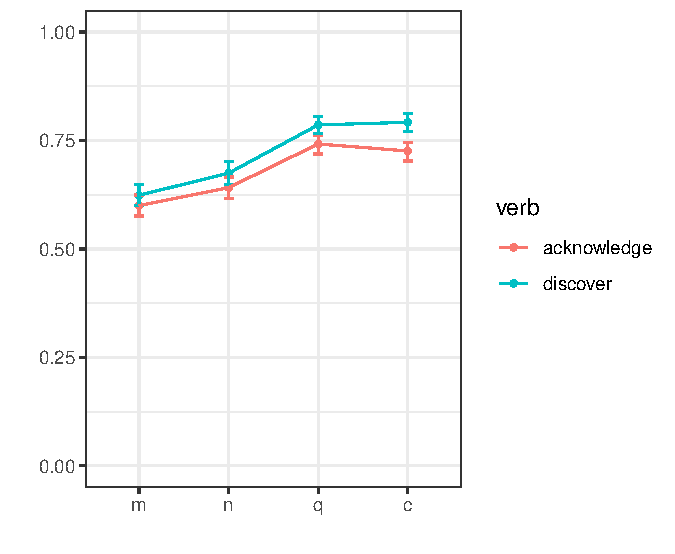
\includegraphics[width=.32\linewidth]{graphs/profile3.pdf}\\
		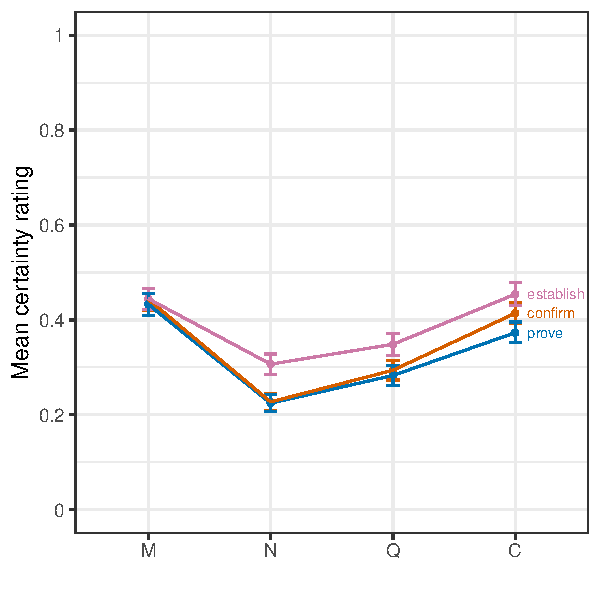
\includegraphics[width=.24\linewidth]{graphs/profile4.pdf}
		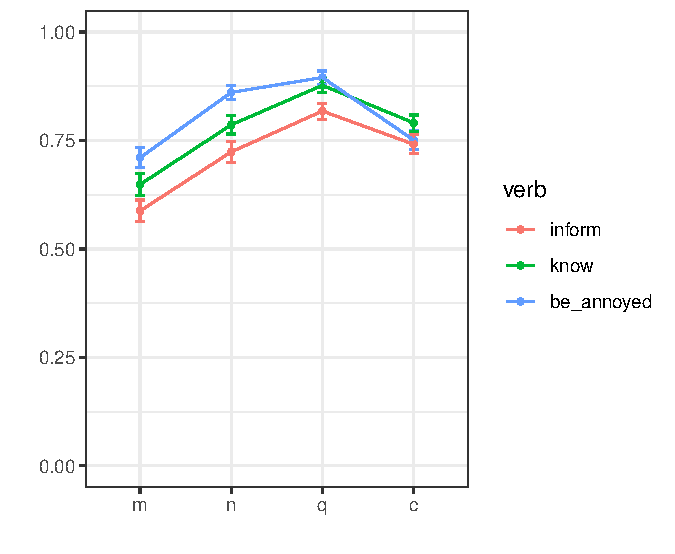
\includegraphics[width=.24\linewidth]{graphs/profile5.pdf}
	\end{minipage}
	\vspace{-\baselineskip}
	\caption{Mean certainty-ratings by operator for four predicate patterns in our data.}
	\label{fig:figure2}
\end{figure}

\newpage

% \begin{table}[ht]
% 	\caption{Model output w \texttt{be\_annoyed/n} as baseline}
% 	\label{tab:annoyed-n}
% 	\centering

% 	\begin{tabular}{lrrrrr}
% 		\toprule
% 		  & Estimate & Std. Error & df & t value & Pr(>|t|)\\
% 		\midrule
% 		(Intercept) & 0.8669958 & 0.0114402 & 1479.204 & 75.7850523 & 0.0000000\\
% 		opc & -0.1155850 & 0.0156641 & 26227.368 & -7.3789836 & 0.0000000\\
% 		opm & -0.1564480 & 0.0155858 & 26288.139 & -10.0378702 & 0.0000000\\
% 		opq & 0.0249138 & 0.0143090 & 56826.915 & 1.7411232 & 0.0816674\\
% 		verbsuggest & -0.6162683 & 0.0134941 & 54372.895 & -45.6694112 & 0.0000000\\
% 		\addlinespace
% 		verbacknowledge & -0.2204417 & 0.0134948 & 54373.777 & -16.3352724 & 0.0000000\\
% 		verbadmit & -0.3402430 & 0.0134933 & 54371.874 & -25.2156750 & 0.0000000\\
% 		verbannounce & -0.3607504 & 0.0134931 & 54371.547 & -26.7359958 & 0.0000000\\
% 		verbbe\_right & -0.6638924 & 0.0134936 & 54372.293 & -49.2003974 & 0.0000000\\
% 		verbconfess & -0.3681695 & 0.0134949 & 54373.904 & -27.2820517 & 0.0000000\\
% 		\addlinespace
% 		verbconfirm & -0.6338363 & 0.0134931 & 54371.657 & -46.9746939 & 0.0000000\\
% 		verbdemonstrate & -0.5307026 & 0.0134935 & 54372.157 & -39.3301466 & 0.0000000\\
% 		verbdiscover & -0.1864716 & 0.0134942 & 54372.992 & -13.8186520 & 0.0000000\\
% 		verbestablish & -0.5542561 & 0.0134933 & 54371.853 & -41.0764079 & 0.0000000\\
% 		verbhear & -0.1956794 & 0.0134938 & 54372.473 & -14.5014554 & 0.0000000\\
% 		\addlinespace
% 		verbinform & -0.1374428 & 0.0134945 & 54373.345 & -10.1851106 & 0.0000000\\
% 		verbknow & -0.0748953 & 0.0134936 & 54372.288 & -5.5504197 & 0.0000000\\
% 		verbpretend & -0.5049533 & 0.0134944 & 54373.218 & -37.4195409 & 0.0000000\\
% 		verbprove & -0.6364950 & 0.0134935 & 54372.138 & -47.1704273 & 0.0000000\\
% 		verbreveal & -0.3057814 & 0.0134937 & 54372.418 & -22.6609884 & 0.0000000\\
% 		\addlinespace
% 		verbsay & -0.5419725 & 0.0134925 & 54370.770 & -40.1685159 & 0.0000000\\
% 		verbsee & -0.1827512 & 0.0134932 & 54371.791 & -13.5438968 & 0.0000000\\
% 		verbthink & -0.5101198 & 0.0134930 & 54371.491 & -37.8062103 & 0.0000000\\
% 		opc:verbsuggest & 0.1594325 & 0.0190634 & 54372.626 & 8.3632939 & 0.0000000\\
% 		opm:verbsuggest & 0.1766113 & 0.0189718 & 54372.046 & 9.3091498 & 0.0000000\\
% 		\addlinespace
% 		opq:verbsuggest & -0.0737648 & 0.0192906 & 54372.717 & -3.8238781 & 0.0001315\\
% 		opc:verbacknowledge & 0.1945569 & 0.0190630 & 54372.333 & 10.2059764 & 0.0000000\\
% 		opm:verbacknowledge & 0.1100553 & 0.0189729 & 54373.070 & 5.8006461 & 0.0000000\\
% 		opq:verbacknowledge & 0.0672935 & 0.0192909 & 54372.991 & 3.4883599 & 0.0004864\\
% 		opc:verbadmit & 0.2803349 & 0.0190626 & 54371.933 & 14.7060204 & 0.0000000\\
% 		\addlinespace
% 		opm:verbadmit & 0.1810708 & 0.0189717 & 54371.994 & 9.5442376 & 0.0000000\\
% 		opq:verbadmit & 0.0440050 & 0.0192896 & 54371.832 & 2.2812856 & 0.0225354\\
% 		opc:verbannounce & 0.2503929 & 0.0190639 & 54373.132 & 13.1343759 & 0.0000000\\
% 		opm:verbannounce & 0.1633026 & 0.0189721 & 54372.338 & 8.6075049 & 0.0000000\\
% 		opq:verbannounce & 0.0017532 & 0.0192899 & 54372.121 & 0.0908892 & 0.9275810\\
% 		\addlinespace
% 		opc:verbbe\_right & 0.1424317 & 0.0190623 & 54371.698 & 7.4718895 & 0.0000000\\
% 		opm:verbbe\_right & 0.2582399 & 0.0189717 & 54371.967 & 13.6118412 & 0.0000000\\
% 		opq:verbbe\_right & -0.0776846 & 0.0192897 & 54371.974 & -4.0272512 & 0.0000565\\
% 		opc:verbconfess & 0.3111230 & 0.0190643 & 54373.455 & 16.3196605 & 0.0000000\\
% 		opm:verbconfess & 0.1837114 & 0.0189741 & 54374.125 & 9.6821973 & 0.0000000\\
% 		\addlinespace
% 		opq:verbconfess & 0.0393640 & 0.0192890 & 54371.320 & 2.0407459 & 0.0412809\\
% 		opc:verbconfirm & 0.2963833 & 0.0190629 & 54372.237 & 15.5476205 & 0.0000000\\
% 		opm:verbconfirm & 0.3663333 & 0.0189721 & 54372.324 & 19.3090505 & 0.0000000\\
% 		opq:verbconfirm & 0.0312870 & 0.0192902 & 54372.377 & 1.6219108 & 0.1048282\\
% 		opc:verbdemonstrate & 0.2854366 & 0.0190647 & 54373.829 & 14.9719656 & 0.0000000\\
% 		\addlinespace
% 		opm:verbdemonstrate & 0.2783816 & 0.0189716 & 54371.830 & 14.6736292 & 0.0000000\\
% 		opq:verbdemonstrate & 0.0753554 & 0.0192892 & 54371.520 & 3.9066023 & 0.0000937\\
% 		opc:verbdiscover & 0.2270099 & 0.0190632 & 54372.450 & 11.9082962 & 0.0000000\\
% 		opm:verbdiscover & 0.1002424 & 0.0189726 & 54372.795 & 5.2835252 & 0.0000001\\
% 		opq:verbdiscover & 0.0762282 & 0.0192898 & 54372.014 & 3.9517423 & 0.0000777\\
% 		\addlinespace
% 		opc:verbestablish & 0.2570817 & 0.0190633 & 54372.539 & 13.4857080 & 0.0000000\\
% 		opm:verbestablish & 0.2879581 & 0.0189714 & 54371.677 & 15.1785426 & 0.0000000\\
% 		opq:verbestablish & 0.0061604 & 0.0192893 & 54371.583 & 0.3193687 & 0.7494481\\
% 		opc:verbhear & 0.2016309 & 0.0190630 & 54372.273 & 10.5770983 & 0.0000000\\
% 		opm:verbhear & -0.0046313 & 0.0189714 & 54371.681 & -0.2441216 & 0.8071376\\
% 		\addlinespace
% 		opq:verbhear & 0.0756021 & 0.0192902 & 54372.373 & 3.9192008 & 0.0000890\\
% 		opc:verbinform & 0.1278740 & 0.0190645 & 54373.631 & 6.7074362 & 0.0000000\\
% 		opm:verbinform & 0.0141486 & 0.0189741 & 54374.122 & 0.7456761 & 0.4558664\\
% 		opq:verbinform & 0.0587564 & 0.0192913 & 54373.322 & 3.0457537 & 0.0023221\\
% 		opc:verbknow & 0.1142699 & 0.0190629 & 54372.206 & 5.9943629 & 0.0000000\\
% 		\addlinespace
% 		opm:verbknow & 0.0130032 & 0.0189709 & 54371.181 & 0.6854301 & 0.4930755\\
% 		opq:verbknow & 0.0569598 & 0.0192897 & 54371.975 & 2.9528579 & 0.0031498\\
% 		opc:verbpretend & -0.0902047 & 0.0190640 & 54373.155 & -4.7316842 & 0.0000022\\
% 		opm:verbpretend & -0.0194245 & 0.0189738 & 54373.822 & -1.0237558 & 0.3059552\\
% 		opq:verbpretend & -0.2196823 & 0.0192900 & 54372.250 & -11.3883795 & 0.0000000\\
% 		\addlinespace
% 		opc:verbprove & 0.2579585 & 0.0190627 & 54372.031 & 13.5320999 & 0.0000000\\
% 		opm:verbprove & 0.3580525 & 0.0189720 & 54372.223 & 18.8726898 & 0.0000000\\
% 		opq:verbprove & 0.0230805 & 0.0192908 & 54372.899 & 1.1964509 & 0.2315259\\
% 		opc:verbreveal & 0.2902650 & 0.0190644 & 54373.511 & 15.2255216 & 0.0000000\\
% 		opm:verbreveal & 0.1767476 & 0.0189723 & 54372.513 & 9.3160804 & 0.0000000\\
% 		\addlinespace
% 		opq:verbreveal & 0.0665887 & 0.0192906 & 54372.717 & 3.4518763 & 0.0005571\\
% 		opc:verbsay & 0.1985351 & 0.0190618 & 54371.193 & 10.4153412 & 0.0000000\\
% 		opm:verbsay & 0.1451974 & 0.0189723 & 54372.495 & 7.6531273 & 0.0000000\\
% 		opq:verbsay & -0.1815738 & 0.0192889 & 54371.195 & -9.4133926 & 0.0000000\\
% 		opc:verbsee & 0.2175191 & 0.0190629 & 54372.234 & 11.4105822 & 0.0000000\\
% 		\addlinespace
% 		opm:verbsee & 0.0594092 & 0.0189723 & 54372.499 & 3.1313655 & 0.0017409\\
% 		opq:verbsee & 0.1108274 & 0.0192896 & 54371.840 & 5.7454526 & 0.0000000\\
% 		opc:verbthink & 0.0023197 & 0.0190619 & 54371.272 & 0.1216913 & 0.9031440\\
% 		opm:verbthink & 0.0145577 & 0.0189717 & 54371.965 & 0.7673367 & 0.4428847\\
% 		opq:verbthink & -0.1738342 & 0.0192903 & 54372.438 & -9.0115053 & 0.0000000\\
% 		\bottomrule
% 	\end{tabular}
% \end{table}

% \newpage

% \begin{table}[ht]
% 	\caption{Model output w \texttt{discover/n} as baseline}
% 	\label{tab:discover-n}
% 	\centering

% 	\begin{tabular}{lrrrrr}
% 		\toprule
% 		  & Estimate & Std. Error & df & t value & Pr(>|t|)\\
% 		\midrule
% 		(Intercept) & 0.6805242 & 0.0114403 & 1479.217 & 59.4849565 & 0.0000000\\
% 		opc & 0.1114249 & 0.0156639 & 26226.686 & 7.1134644 & 0.0000000\\
% 		opm & -0.0562056 & 0.0155855 & 26286.826 & -3.6062779 & 0.0003112\\
% 		opq & 0.1011420 & 0.0143103 & 56828.295 & 7.0677830 & 0.0000000\\
% 		verbbe\_annoyed & 0.1864716 & 0.0134942 & 54372.998 & 13.8186521 & 0.0000000\\
% 		\addlinespace
% 		verbsuggest & -0.4297967 & 0.0134937 & 54372.361 & -31.8516905 & 0.0000000\\
% 		verbacknowledge & -0.0339702 & 0.0134936 & 54372.308 & -2.5174950 & 0.0118221\\
% 		verbadmit & -0.1537714 & 0.0134942 & 54372.985 & -11.3953857 & 0.0000000\\
% 		verbannounce & -0.1742788 & 0.0134947 & 54373.649 & -12.9145926 & 0.0000000\\
% 		verbbe\_right & -0.4774208 & 0.0134935 & 54372.079 & -35.3816304 & 0.0000000\\
% 		\addlinespace
% 		verbconfess & -0.1816980 & 0.0134936 & 54372.192 & -13.4655376 & 0.0000000\\
% 		verbconfirm & -0.4473648 & 0.0134944 & 54373.311 & -33.1517710 & 0.0000000\\
% 		verbdemonstrate & -0.3442310 & 0.0134928 & 54371.247 & -25.5121517 & 0.0000000\\
% 		verbestablish & -0.3677846 & 0.0134928 & 54371.167 & -27.2579106 & 0.0000000\\
% 		verbhear & -0.0092079 & 0.0134940 & 54372.798 & -0.6823676 & 0.4950095\\
% 		\addlinespace
% 		verbinform & 0.0490288 & 0.0134942 & 54373.066 & 3.6333114 & 0.0002801\\
% 		verbknow & 0.1115762 & 0.0134931 & 54371.668 & 8.2691029 & 0.0000000\\
% 		verbpretend & -0.3184818 & 0.0134943 & 54373.176 & -23.6011440 & 0.0000000\\
% 		verbprove & -0.4500234 & 0.0134934 & 54372.042 & -33.3512833 & 0.0000000\\
% 		verbreveal & -0.1193099 & 0.0134941 & 54372.880 & -8.8416323 & 0.0000000\\
% 		\addlinespace
% 		verbsay & -0.3555009 & 0.0134943 & 54373.168 & -26.3444678 & 0.0000000\\
% 		verbsee & 0.0037204 & 0.0134930 & 54371.450 & 0.2757288 & 0.7827574\\
% 		verbthink & -0.3236483 & 0.0134936 & 54372.197 & -23.9853913 & 0.0000000\\
% 		opc:verbbe\_annoyed & -0.2270099 & 0.0190632 & 54372.453 & -11.9082963 & 0.0000000\\
% 		opm:verbbe\_annoyed & -0.1002424 & 0.0189726 & 54372.798 & -5.2835253 & 0.0000001\\
% 		\addlinespace
% 		opq:verbbe\_annoyed & -0.0762282 & 0.0192898 & 54372.017 & -3.9517423 & 0.0000777\\
% 		opc:verbsuggest & -0.0675773 & 0.0190625 & 54371.851 & -3.5450396 & 0.0003929\\
% 		opm:verbsuggest & 0.0763690 & 0.0189709 & 54371.211 & 4.0255864 & 0.0000569\\
% 		opq:verbsuggest & -0.1499930 & 0.0192910 & 54373.069 & -7.7752981 & 0.0000000\\
% 		opc:verbacknowledge & -0.0324529 & 0.0190617 & 54371.116 & -1.7025196 & 0.0886637\\
% 		\addlinespace
% 		opm:verbacknowledge & 0.0098129 & 0.0189711 & 54371.417 & 0.5172570 & 0.6049789\\
% 		opq:verbacknowledge & -0.0089347 & 0.0192902 & 54372.396 & -0.4631724 & 0.6432426\\
% 		opc:verbadmit & 0.0533251 & 0.0190632 & 54372.508 & 2.7972739 & 0.0051554\\
% 		opm:verbadmit & 0.0808284 & 0.0189728 & 54372.916 & 4.2602367 & 0.0000205\\
% 		opq:verbadmit & -0.0322232 & 0.0192908 & 54372.883 & -1.6703960 & 0.0948468\\
% 		\addlinespace
% 		opc:verbannounce & 0.0233831 & 0.0190642 & 54373.367 & 1.2265427 & 0.2199998\\
% 		opm:verbannounce & 0.0630602 & 0.0189726 & 54372.754 & 3.3237576 & 0.0008887\\
% 		opq:verbannounce & -0.0744750 & 0.0192926 & 54374.465 & -3.8602856 & 0.0001134\\
% 		opc:verbbe\_right & -0.0845782 & 0.0190620 & 54371.360 & -4.4370099 & 0.0000091\\
% 		opm:verbbe\_right & 0.1579976 & 0.0189719 & 54372.163 & 8.3279685 & 0.0000000\\
% 		\addlinespace
% 		opq:verbbe\_right & -0.1539128 & 0.0192901 & 54372.283 & -7.9788617 & 0.0000000\\
% 		opc:verbconfess & 0.0841131 & 0.0190632 & 54372.437 & 4.4123417 & 0.0000102\\
% 		opm:verbconfess & 0.0834691 & 0.0189719 & 54372.142 & 4.3996174 & 0.0000109\\
% 		opq:verbconfess & -0.0368642 & 0.0192905 & 54372.632 & -1.9110088 & 0.0560087\\
% 		opc:verbconfirm & 0.0693734 & 0.0190644 & 54373.529 & 3.6388992 & 0.0002741\\
% 		\addlinespace
% 		opm:verbconfirm & 0.2660910 & 0.0189728 & 54372.917 & 14.0248948 & 0.0000000\\
% 		opq:verbconfirm & -0.0449413 & 0.0192914 & 54373.472 & -2.3295974 & 0.0198311\\
% 		opc:verbdemonstrate & 0.0584268 & 0.0190633 & 54372.586 & 3.0648793 & 0.0021786\\
% 		opm:verbdemonstrate & 0.1781393 & 0.0189714 & 54371.707 & 9.3898743 & 0.0000000\\
% 		opq:verbdemonstrate & -0.0008729 & 0.0192906 & 54372.707 & -0.0452486 & 0.9639093\\
% 		\addlinespace
% 		opc:verbestablish & 0.0300718 & 0.0190618 & 54371.161 & 1.5775980 & 0.1146638\\
% 		opm:verbestablish & 0.1877158 & 0.0189720 & 54372.212 & 9.8943713 & 0.0000000\\
% 		opq:verbestablish & -0.0700678 & 0.0192899 & 54372.103 & -3.6323635 & 0.0002811\\
% 		opc:verbhear & -0.0253789 & 0.0190637 & 54372.970 & -1.3312665 & 0.1831069\\
% 		opm:verbhear & -0.1048737 & 0.0189721 & 54372.368 & -5.5277707 & 0.0000000\\
% 		\addlinespace
% 		opq:verbhear & -0.0006261 & 0.0192909 & 54372.991 & -0.0324581 & 0.9741069\\
% 		opc:verbinform & -0.0991359 & 0.0190633 & 54372.605 & -5.2003420 & 0.0000002\\
% 		opm:verbinform & -0.0860938 & 0.0189733 & 54373.368 & -4.5376355 & 0.0000057\\
% 		opq:verbinform & -0.0174718 & 0.0192931 & 54374.843 & -0.9055994 & 0.3651520\\
% 		opc:verbknow & -0.1127399 & 0.0190628 & 54372.127 & -5.9141311 & 0.0000000\\
% 		\addlinespace
% 		opm:verbknow & -0.0872392 & 0.0189719 & 54372.149 & -4.5983336 & 0.0000043\\
% 		opq:verbknow & -0.0192684 & 0.0192895 & 54371.814 & -0.9989027 & 0.3178463\\
% 		opc:verbpretend & -0.3172145 & 0.0190639 & 54373.134 & -16.6395086 & 0.0000000\\
% 		opm:verbpretend & -0.1196669 & 0.0189725 & 54372.658 & -6.3073967 & 0.0000000\\
% 		opq:verbpretend & -0.2959105 & 0.0192916 & 54373.627 & -15.3388172 & 0.0000000\\
% 		\addlinespace
% 		opc:verbprove & 0.0309486 & 0.0190626 & 54371.908 & 1.6235265 & 0.1044827\\
% 		opm:verbprove & 0.2578102 & 0.0189728 & 54372.987 & 13.5883819 & 0.0000000\\
% 		opq:verbprove & -0.0531478 & 0.0192907 & 54372.839 & -2.7550974 & 0.0058694\\
% 		opc:verbreveal & 0.0632551 & 0.0190641 & 54373.234 & 3.3180321 & 0.0009071\\
% 		opm:verbreveal & 0.0765052 & 0.0189711 & 54371.383 & 4.0327309 & 0.0000552\\
% 		\addlinespace
% 		opq:verbreveal & -0.0096396 & 0.0192917 & 54373.669 & -0.4996755 & 0.6173056\\
% 		opc:verbsay & -0.0284748 & 0.0190633 & 54372.590 & -1.4936938 & 0.1352615\\
% 		opm:verbsay & 0.0449550 & 0.0189713 & 54371.586 & 2.3696339 & 0.0178092\\
% 		opq:verbsay & -0.2578020 & 0.0192911 & 54373.227 & -13.3637456 & 0.0000000\\
% 		opc:verbsee & -0.0094907 & 0.0190633 & 54372.613 & -0.4978528 & 0.6185898\\
% 		\addlinespace
% 		opm:verbsee & -0.0408332 & 0.0189714 & 54371.728 & -2.1523480 & 0.0313743\\
% 		opq:verbsee & 0.0345992 & 0.0192916 & 54373.623 & 1.7934827 & 0.0729013\\
% 		opc:verbthink & -0.2246902 & 0.0190628 & 54372.159 & -11.7868151 & 0.0000000\\
% 		opm:verbthink & -0.0856847 & 0.0189719 & 54372.175 & -4.5163904 & 0.0000063\\
% 		opq:verbthink & -0.2500624 & 0.0192911 & 54373.178 & -12.9625865 & 0.0000000\\
% 		\bottomrule
% 	\end{tabular}
% \end{table}

% \newpage

% \begin{table}[ht]
% 	\caption{Model output w \texttt{know/n} as baseline}
% 	\label{tab:discover-n}
% 	\centering

% 	\begin{tabular}{lrrrrr}
% 		\toprule
% 		  & Estimate & Std. Error & df & t value & Pr(>|t|)\\
% 		\midrule
% 		(Intercept) & 0.7921005 & 0.0114401 & 1479.182 & 69.2391632 & 0.0000000\\
% 		opc & -0.0013151 & 0.0156638 & 26226.099 & -0.0839558 & 0.9330922\\
% 		opm & -0.1434448 & 0.0155855 & 26286.727 & -9.2037503 & 0.0000000\\
% 		opq & 0.0818736 & 0.0143093 & 56827.205 & 5.7217106 & 0.0000000\\
% 		verbdiscover & -0.1115762 & 0.0134931 & 54371.661 & -8.2691029 & 0.0000000\\
% 		\addlinespace
% 		verbbe\_annoyed & 0.0748953 & 0.0134936 & 54372.286 & 5.5504198 & 0.0000000\\
% 		verbsuggest & -0.5413729 & 0.0134928 & 54371.215 & -40.1230775 & 0.0000000\\
% 		verbacknowledge & -0.1455464 & 0.0134940 & 54372.778 & -10.7859911 & 0.0000000\\
% 		verbadmit & -0.2653476 & 0.0134936 & 54372.243 & -19.6647018 & 0.0000000\\
% 		verbannounce & -0.2858550 & 0.0134935 & 54372.051 & -21.1847253 & 0.0000000\\
% 		\addlinespace
% 		verbbe\_right & -0.5889971 & 0.0134936 & 54372.234 & -43.6501264 & 0.0000000\\
% 		verbconfess & -0.2932742 & 0.0134933 & 54371.896 & -21.7347532 & 0.0000000\\
% 		verbconfirm & -0.5589410 & 0.0134943 & 54373.134 & -41.4204989 & 0.0000000\\
% 		verbdemonstrate & -0.4558072 & 0.0134931 & 54371.605 & -33.7807521 & 0.0000000\\
% 		verbestablish & -0.4793608 & 0.0134938 & 54372.501 & -35.5245129 & 0.0000000\\
% 		\addlinespace
% 		verbhear & -0.1207841 & 0.0134931 & 54371.608 & -8.9515418 & 0.0000000\\
% 		verbinform & -0.0625474 & 0.0134940 & 54372.811 & -4.6351853 & 0.0000036\\
% 		verbpretend & -0.4300580 & 0.0134939 & 54372.685 & -31.8704317 & 0.0000000\\
% 		verbprove & -0.5615997 & 0.0134934 & 54372.014 & -41.6202578 & 0.0000000\\
% 		verbreveal & -0.2308861 & 0.0134943 & 54373.179 & -17.1098402 & 0.0000000\\
% 		\addlinespace
% 		verbsay & -0.4670771 & 0.0134939 & 54372.578 & -34.6140392 & 0.0000000\\
% 		verbsee & -0.1078558 & 0.0134932 & 54371.715 & -7.9933523 & 0.0000000\\
% 		verbthink & -0.4352245 & 0.0134933 & 54371.896 & -32.2547883 & 0.0000000\\
% 		opc:verbdiscover & 0.1127399 & 0.0190628 & 54372.122 & 5.9141311 & 0.0000000\\
% 		opm:verbdiscover & 0.0872392 & 0.0189719 & 54372.145 & 4.5983336 & 0.0000043\\
% 		\addlinespace
% 		opq:verbdiscover & 0.0192684 & 0.0192895 & 54371.810 & 0.9989027 & 0.3178463\\
% 		opc:verbbe\_annoyed & -0.1142699 & 0.0190629 & 54372.206 & -5.9943630 & 0.0000000\\
% 		opm:verbbe\_annoyed & -0.0130032 & 0.0189709 & 54371.180 & -0.6854301 & 0.4930755\\
% 		opq:verbbe\_annoyed & -0.0569598 & 0.0192897 & 54371.974 & -2.9528580 & 0.0031498\\
% 		opc:verbsuggest & 0.0451626 & 0.0190614 & 54370.865 & 2.3693169 & 0.0178244\\
% 		\addlinespace
% 		opm:verbsuggest & 0.1636081 & 0.0189713 & 54371.561 & 8.6239932 & 0.0000000\\
% 		opq:verbsuggest & -0.1307246 & 0.0192896 & 54371.847 & -6.7769511 & 0.0000000\\
% 		opc:verbacknowledge & 0.0802870 & 0.0190639 & 54373.059 & 4.2114778 & 0.0000254\\
% 		opm:verbacknowledge & 0.0970521 & 0.0189731 & 54373.215 & 5.1152465 & 0.0000003\\
% 		opq:verbacknowledge & 0.0103337 & 0.0192900 & 54372.183 & 0.5357031 & 0.5921659\\
% 		\addlinespace
% 		opc:verbadmit & 0.1660650 & 0.0190633 & 54372.568 & 8.7112405 & 0.0000000\\
% 		opm:verbadmit & 0.1680676 & 0.0189725 & 54372.674 & 8.8584875 & 0.0000000\\
% 		opq:verbadmit & -0.0129548 & 0.0192897 & 54371.901 & -0.6715939 & 0.5018451\\
% 		opc:verbannounce & 0.1361230 & 0.0190629 & 54372.249 & 7.1407107 & 0.0000000\\
% 		opm:verbannounce & 0.1502994 & 0.0189716 & 54371.859 & 7.9223393 & 0.0000000\\
% 		\addlinespace
% 		opq:verbannounce & -0.0552066 & 0.0192897 & 54371.911 & -2.8619784 & 0.0042117\\
% 		opc:verbbe\_right & 0.0281618 & 0.0190625 & 54371.883 & 1.4773357 & 0.1395915\\
% 		opm:verbbe\_right & 0.2452367 & 0.0189720 & 54372.236 & 12.9262410 & 0.0000000\\
% 		opq:verbbe\_right & -0.1346444 & 0.0192901 & 54372.308 & -6.9799743 & 0.0000000\\
% 		opc:verbconfess & 0.1968531 & 0.0190627 & 54372.016 & 10.3266157 & 0.0000000\\
% 		\addlinespace
% 		opm:verbconfess & 0.1707082 & 0.0189737 & 54373.731 & 8.9971020 & 0.0000000\\
% 		opq:verbconfess & -0.0175959 & 0.0192891 & 54371.441 & -0.9122160 & 0.3616590\\
% 		opc:verbconfirm & 0.1821133 & 0.0190626 & 54371.955 & 9.5534239 & 0.0000000\\
% 		opm:verbconfirm & 0.3533301 & 0.0189718 & 54372.046 & 18.6239655 & 0.0000000\\
% 		opq:verbconfirm & -0.0256729 & 0.0192917 & 54373.707 & -1.3307729 & 0.1832693\\
% 		\addlinespace
% 		opc:verbdemonstrate & 0.1711667 & 0.0190647 & 54373.791 & 8.9782020 & 0.0000000\\
% 		opm:verbdemonstrate & 0.2653784 & 0.0189716 & 54371.911 & 13.9881581 & 0.0000000\\
% 		opq:verbdemonstrate & 0.0183955 & 0.0192903 & 54372.499 & 0.9536136 & 0.3402835\\
% 		opc:verbestablish & 0.1428117 & 0.0190634 & 54372.667 & 7.4914038 & 0.0000000\\
% 		opm:verbestablish & 0.2749549 & 0.0189719 & 54372.156 & 14.4927310 & 0.0000000\\
% 		\addlinespace
% 		opq:verbestablish & -0.0507994 & 0.0192892 & 54371.529 & -2.6335636 & 0.0084518\\
% 		opc:verbhear & 0.0873610 & 0.0190622 & 54371.557 & 4.5829467 & 0.0000046\\
% 		opm:verbhear & -0.0176345 & 0.0189709 & 54371.193 & -0.9295579 & 0.3526042\\
% 		opq:verbhear & 0.0186422 & 0.0192902 & 54372.432 & 0.9664076 & 0.3338446\\
% 		opc:verbinform & 0.0136041 & 0.0190628 & 54372.117 & 0.7136441 & 0.4754504\\
% 		\addlinespace
% 		opm:verbinform & 0.0011454 & 0.0189738 & 54373.859 & 0.0603655 & 0.9518647\\
% 		opq:verbinform & 0.0017966 & 0.0192921 & 54374.044 & 0.0931259 & 0.9258039\\
% 		opc:verbpretend & -0.2044746 & 0.0190640 & 54373.227 & -10.7256652 & 0.0000000\\
% 		opm:verbpretend & -0.0324277 & 0.0189726 & 54372.773 & -1.7091875 & 0.0874219\\
% 		opq:verbpretend & -0.2766421 & 0.0192909 & 54373.044 & -14.3405213 & 0.0000000\\
% 		\addlinespace
% 		opc:verbprove & 0.1436885 & 0.0190622 & 54371.604 & 7.5378609 & 0.0000000\\
% 		opm:verbprove & 0.3450493 & 0.0189712 & 54371.500 & 18.1880552 & 0.0000000\\
% 		opq:verbprove & -0.0338794 & 0.0192909 & 54373.040 & -1.7562330 & 0.0790543\\
% 		opc:verbreveal & 0.1759951 & 0.0190637 & 54372.960 & 9.2319255 & 0.0000000\\
% 		opm:verbreveal & 0.1637444 & 0.0189722 & 54372.374 & 8.6307727 & 0.0000000\\
% 		\addlinespace
% 		opq:verbreveal & 0.0096288 & 0.0192902 & 54372.406 & 0.4991553 & 0.6176720\\
% 		opc:verbsay & 0.0842652 & 0.0190632 & 54372.497 & 4.4203002 & 0.0000099\\
% 		opm:verbsay & 0.1321942 & 0.0189719 & 54372.094 & 6.9679113 & 0.0000000\\
% 		opq:verbsay & -0.2385336 & 0.0192898 & 54371.999 & -12.3658155 & 0.0000000\\
% 		opc:verbsee & 0.1032492 & 0.0190630 & 54372.324 & 5.4162003 & 0.0000001\\
% 		\addlinespace
% 		opm:verbsee & 0.0464060 & 0.0189718 & 54372.089 & 2.4460454 & 0.0144464\\
% 		opq:verbsee & 0.0538675 & 0.0192901 & 54372.298 & 2.7924979 & 0.0052321\\
% 		opc:verbthink & -0.1119503 & 0.0190627 & 54372.030 & -5.8727378 & 0.0000000\\
% 		opm:verbthink & 0.0015545 & 0.0189713 & 54371.557 & 0.0819391 & 0.9346955\\
% 		opq:verbthink & -0.2307940 & 0.0192903 & 54372.447 & -11.9642778 & 0.0000000\\
% 		\bottomrule
% 	\end{tabular}
% \end{table}

\bibliography{projective-content.bib}

\end{document}